\documentclass[main]{subfiles}

\begin{document}

\chapter{Elecci\'on de Hardware}
%\thispagestyle{plain}
%\pagestyle{fancy}


La elecci\'on del Hardware significa una parte muy importante del Proyecto, ya que las decisiones tomadas condicionan el resto del mismo. Una mala elecci\'on de alguno de los componentes puede resultar en complicaciones no previstas a la hora de la ejecuci\'on, causando contratiempos inesperados y trabajo excesivo. Es necesario, entonces, el estudio detallado de cada uno de los componentes a utilizar, comparando caracter\'isticas, rendimientos y utilidades. \\
Elegir adecuadamente el Hardware necesario agiliza las etapas siguientes de todo el Proyecto. Resulta fundamental la toma de buenas decisiones, las cuales deben estar basadas en un previo estudio de cada etapa del proyecto, sus requerimientos, un estudio comparativo de las posibles soluciones y el conocimiento cabal de los componentes a utilizar.\\

\section{Elecci\'on de plataforma f\'isica: Cuadric\'opteros}
\vspace*{15pt}

A la hora de la planificaci\'on del Proyecto se plantean dos opciones que se diferencian b\'asicamente en el punto de partida. Ambas tienen como objetivo principal dise\~nar e integrar un sistema de control que permita al cuadric\'optero mantener un vuelo aut\'onomo, pero una de ellas consta adem\'as del dise\~no y el armado del mismo. \\Esta \'ultima incluye desaf\'ios de ingenier\'ia mec\'anica, conocimientos de resistencia, flexibilidad y peso de materiales, as\'i como tambi\'en diversas complicaciones a la hora de fabricar y armar las partes. \\ Teniendo en cuenta que se trata de un proyecto con tiempo acotado y su objetivo se centra en el control del veh\'iculo, la necesidad de partir de hardware ya construido resulta imperiosa. Por ello se realiza un estudio sobre las opciones que el mercado ofrece en esta materia. Desafortunadamente, las opciones no son muy numerosas, disponiendo de cuadric\'opteros comerciales controlados a control remoto. Todos ellos incluyen un peque\~no sistema de control integrado del cu\'al no es posible obtener informaci\'on, ya que se trata de software privativo. Las opciones que el mercado ofrece son: 
\begin{itemize}
	\item Gaui 330X
	\item XAircraft X650
	\item Turbo Ace X720
\end{itemize}
Se procede a la comparaci\'on de los equipos mencionados y se analizan algunos aspectos fundamentales y cr\'iticos, como puede ser por ejemplo el peso del dispositivo y la carga \'util que puede soportar.\\[20pt]

\subsubsection*{Motor}
Al estudiar las posibilidades nos encontramos con que en todos los casos los motores se controlan con modulaci\'on por ancho de pulsos, de ahora en m\'as \textbf{PWM} por sus siglas en ingl\'es, t\'ecnica en la cual se modifica el ciclo de trabajo de una se\~nal peri\'odica para controlar la cantidad de energ\'ia que se entrega a una carga.\\

	En la tabla \ref{tab:motor} se muestran las caracter\'isticas de los motores de los 3 cuadric\'opteros considerados.\\

\begin{table}[H]
\begin{tabular}{p{40pt}|p{80pt}|p{130pt}|p{130pt}|} 
\cline{2-4}
& \cellcolor[gray]{0.8} \textbf{GAUI 330X} 
& \cellcolor[gray]{0.8} \textbf{XAircraft X650} 
& \cellcolor[gray]{0.8} \textbf{Turbo Ace X720} \\ \cline{2-4} \hline
\multicolumn{1}{|p{40pt}|}{\cellcolor[gray]{0.8}\textbf{Motor}} 
& H\'elices de 8 pulgadas, 4 motores brushless con 4 ESCs de 10A 
& H\'elices de 12 pulgadas, 4 motores brushless con 4 ESCs de 10A. Las h\'elices impulsadas por el motor tienen una eficiencia de 9g/W bajo carga nominal. 
& H\'elices de 12 pulgadas, 4 motores brushless con 4 ESCs de 10A. Las h\'elices impulsadas por el motor tienen una eficiencia de 12g/W bajo carga nominal.\\ \hline
\end{tabular} 
\caption{Comparaci\'on motores}
\label{tab:motor}
\end{table}

	Los motores \emph{Brushless} son motores el\'ectricos alimentados con corriente continua. Tienen un sistema de conmutaci\'on el\'ectrico y presentan relaciones lineales entre \emph{Corriente} y \emph{Torque} y entre \emph{Frecuencia} y \emph{velocidad}. Son com\'unmente utilizados en veh\'iculos radio-controlados por su gran eficiencia, potencia, durabilidad y su bajo peso en comparaci\'on con los tradicionales motores \emph{Brushed}. Sin embargo, los motores de CC \emph{Brushless} son mucho m\'as complicados de controlar, ya que la fase var\'ia con la rotaci\'on del motor. Para controlarlos debe utilizarse un dispositivo llamado \emph{Controlador el\'ectrico de velocidad}, o \textbf{ESCs}. Com\'unmente los ESCs se clasifican seg\'un su corriente m\'axima, por ejemplo 10 amp\'eres o 10A.\\

	Como se puede ver en la tabla \ref{tab:motor}, todos los dispositivos utilizan motores similares y la \'unica diferencia radica en que la eficiencia de los motores del \emph{Turbo Ace X720} es mayor.

\subsubsection*{Tiempo de vuelo}

	El tiempo de vuelo puede resultar cr\'itico seg\'un la aplicaci\'on considerada. En la tabla \ref{tab:tiempo} se muestran los datos que se obtuvieron para los 3 cuadric\'opteros considerados.

\begin{table}[H]
\begin{tabular}{p{40pt}|p{80pt}|p{130pt}|p{130pt}|} 
\cline{2-4}
& \cellcolor[gray]{0.8} \textbf{GAUI 330X} 
& \cellcolor[gray]{0.8} \textbf{XAircraft X650} 
& \cellcolor[gray]{0.8} \textbf{Turbo Ace X720} \\ \cline{2-4} \hline
\multicolumn{1}{|p{40pt}|}{\cellcolor[gray]{0.8}\textbf{Tiempo de vuelo}} 
& Con bater\'ia de $2200 mAh$ vuela entre 7 y 20 minutos & Vuela 12 minutos con bater\'ia de $2200mAh$ y carga menor a $1.5kg$ & Con bater\'ia de $2200mAh$ vuela 15 minutos a carga nominal y puede llegar a la media hora de vuelo con una bater\'ia de $10.000mAh$ \\ \hline
\end{tabular}
\caption{Comparaci\'on Tiempo de vuelo}
\label{tab:tiempo}
\end{table}

	Como se puede apreciar los tiempos de vuelo son similares en los 3 dspositivos, por lo que no ser\'a un factor determinante a la hora de tomar la decisi\'on.\\

	Un factor determinante en el tiempo de vuelo es la bater\'ia a utilizar. Deben considerarse 2 aspectos importantes: la capacidad de la bater\'ia y su peso. Si bien una bater\'ia con mayor capacidad permitir\'a mayor autonom\'ia de vuelo, es claro que su peso tambi\'en aumentar\'a, lo cual a su vez, causar\'a un mayor consumo. Los 3 cuadric\'opteros en consideraci\'on incluyen una bater\'ia de 3 celdas de Litio de $2200 \, mAh$.

\subsubsection*{Peso}

	La carga \'util que el dispositivo pueda soportar juega un papel fundamental. Vale recordar que, adem\'as de toda la instrumentaci\'on que incluye el cuadric\'optero, se incorporar\'a un microprocesador, una bater\'ia independiente para su alimentaci\'on, un gir\'oscopo, un aceler\'ometro, un GPS y alguna interfaz para la comunicaci\'on. A su vez es interesante conservar la posibilidad de integrar una c\'amara fotogr\'afica convencional ya que puede ser de gran utilidad para numerosas aplicaciones. La fuerza que los motores pueden realizar es acotada, por lo que el peso del dispositivo influye directamente en la carga \'util del mismo.

\begin{table}[H]
\begin{tabular}{p{40pt}|p{70pt}|p{160pt}|p{110pt}|} 
\cline{2-4}
& \cellcolor[gray]{0.8} \textbf{GAUI 330X} 
& \cellcolor[gray]{0.8} \textbf{XAircraft X650} 
& \cellcolor[gray]{0.8} \textbf{Turbo Ace X720} \\ \cline{2-4} \hline
\multicolumn{1}{|p{40pt}|}{\cellcolor[gray]{0.8}\textbf{Peso}} 
& $700g$ & Versi\'on de fibra de vidrio: $1100g$. Versi\'on de fibra de carbono: $950g$. & $990g$ \\ \hline
\multicolumn{1}{|p{40pt}|}{\cellcolor[gray]{0.8}\textbf{Carga \'util}} 
& $500g$ & Versi\'on de fibra de vidrio: $700g$. Versi\'on de fibra de carbono: $850g$. & $1300 g$ \\ 
\hline 
\end{tabular}
\caption{Comparaci\'on peso y carga \'util}
\label{tab:peso}
\end{table}

Como se puede ver en la tabla \ref{tab:peso}, no cabe duda que el dispositivo que puede cargar con m\'as peso es el \emph{Turbo Ace X720}, lo cual constituye una ventaja considerable de este dispositivo frente a los otros.

\subsubsection*{Instrumentaci\'on}

	Toda la instrumentaci\'on que los dispositivos brindan est\'a originalmente destinada al manejo mediante el control remoto. Todos ellos incluyen un aceler\'ometro y un gir\'oscopo de 3 ejes y traen alg\'un sistema de estabilizaci\'on incluido, de forma tal de facilitar el control. \\

	Como ya se mencion\'o, se a\~nadir\'a al cuadric\'optero la instrumentaci\'on necesaria para su control autom\'atico, por lo cual la instrumentaci\'on incluida en el dispositivo carece de gran importancia. Sin embargo, resulta interesante conservar la posibilidad de controlarlo mediante el control remoto, ya que puede ser \'util tanto en determinadas aplicaciones, como para evitar eventualidades en las primeras pruebas donde se testean los algoritmos de control desarrollados. El algoritmo de control deber\'a poder alternar entre estos dos modos de vuelo d\'andole prioridad al control remoto, de modo de conservar la integridad f\'isica del dispositivo ante fallas en los algoritmos de control.

\begin{table}[H]
\begin{tabular}{p{40pt}|p{85pt}|p{125pt}|p{130pt}|} 
\cline{2-4}
& \cellcolor[gray]{0.8} \textbf{GAUI 330X} 
& \cellcolor[gray]{0.8} \textbf{XAircraft X650} 
& \cellcolor[gray]{0.8} \textbf{Turbo Ace X720} \\ \cline{2-4} \hline
\multicolumn{1}{|p{40pt}|}{\cellcolor[gray]{0.8}\textbf{Instru- mentaci\'on}} 
& Sistema de estabilizaci\'on integrado \emph{GU344}: incluye gir\'oscopo de 3 ejes y aceler\'ometro. & Gir\'oscopo de 3 ejes y aceler\'ometro. Puede usar hasta 13 sensores para chequiar actitud de vuelo, altitud, direcci\'on, posici\'on, temperatura, consumo energ\'etico, etc. & Gir\'oscopo y aceler\'ometro de 3 ejes integrados. Se vende por separado el m\'odulo GPS que incluye bar\'ometro como medidor de altitud y br\'ujula electr\'onica.\\ 
\hline 
\end{tabular}
\caption{Comparaci\'on instrumentaci\'on}
\label{tab:instrumentacion}
\end{table}

	En la tabla \ref{tab:instrumentacion} se muestra un resumen de la instrumentaci\'on incluida en cada cuadric\'opetro. 

\subsubsection*{Control}

	El control mediante el mando remoto requiere de cierta pr\'actica y habilidad para ejecutarlo de buena forma, por lo cual todos los algoritmos de control integrados que el dispositivo incluya significar\'an una interesante ventaja. Por otro lado se debe tener en cuenta que el control remoto se utilizar\'a en reducidos casos, siendo el control autom\'atico el verdadero inter\'es del proyecto. Es importante tener en cuenta que dichos algoritmos encarecen el precio del dispositivo y no ser\'an utilizados con mucha frecuencia.

\begin{table}[H]
\begin{tabular}{p{40pt}|p{70pt}|p{160pt}|p{110pt}|} 
\cline{2-4}
& \cellcolor[gray]{0.8} \textbf{GAUI 330X} 
& \cellcolor[gray]{0.8} \textbf{XAircraft X650} 
& \cellcolor[gray]{0.8} \textbf{Turbo Ace X720} \\ \cline{2-4} \hline
\multicolumn{1}{|p{40pt}|}{\cellcolor[gray]{0.8}\textbf{Control}} 
& - & Software de configuraci\'on incluido. Dispositivo de control de 4 velocidades dise\~nado todo en 1. Soporta protocolos $Ultra$ $PWM$ y control de frecuencia hasta $500Hz$. Posee algoritmos de control de vuelo incorporados que hacen q sea mas f\'acil volarlo & Nivelaci\'on autom\'atica con control de altitud \\ 
\hline 
\end{tabular}
\caption{Comparaci\'on control}
\label{tab:control}
\end{table}

	Si bien el \emph{XAircraft X650} es el que tiene m\'as algoritmos de control implementados que facilitan su mando, se considera que el dispositivo que se adec\'ua m\'as a nuestras necesidades es el \emph{Turbo Ace X720}. Tiene un peque\~no sistema de estabilizaci\'on que ayuda a la hora de su control, pero no incluye demasiado software ni hardware que no ser\'a utilizado y encarecen al producto, como el \emph{XAircraft X650}.

\subsubsection*{Dimensiones}

	Las dimensiones de los 3 cuadric\'opteros considerados se pueden apreciar en la tabla \ref{tab:dimensiones}.

\begin{table}[H]
\begin{tabular}{p{40pt}|p{80pt}|p{130pt}|p{130pt}|} 
\cline{2-4}
& \cellcolor[gray]{0.8} \textbf{GAUI 330X} 
& \cellcolor[gray]{0.8} \textbf{XAircraft X650} 
& \cellcolor[gray]{0.8} \textbf{Turbo Ace X720} \\ \cline{2-4} \hline
\multicolumn{1}{|p{40pt}|}{\cellcolor[gray]{0.8}\textbf{Dimen- siones}} 
& 33 cm entre ejes diagonalmente opuestos & 61.5 cm entre ejes diagonalmente opuestos & 61.5 cm entre ejes diagonalmente opuestos \\ 
\hline 
\end{tabular}
\caption{Comparaci\'on dimensiones}
\label{tab:dimensiones}
\end{table}

	Como se puede ver el \emph{GAUI} es el m\'as peque\~no, mientras que los otros dos tienen el mismo tama\~no aproximadamente.

	En la figura \ref{fig:cuadricopteros} se pueden apreciar fotograf\'ias de los 3 equipos considerados.

\begin{figure} [h!]
  \centering
  \subfloat[GAUI 330X]{\label{fig:gaui}
  		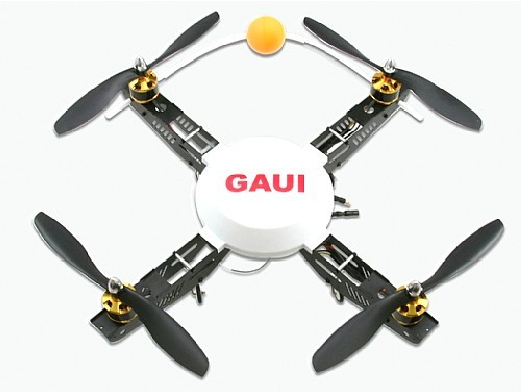
\includegraphics[width=0.3\textwidth]
  			{./pics_eleccion_hardware/gaui.png}}
  \subfloat[XAircraft X650]{\label{fig:aircraft} 
  		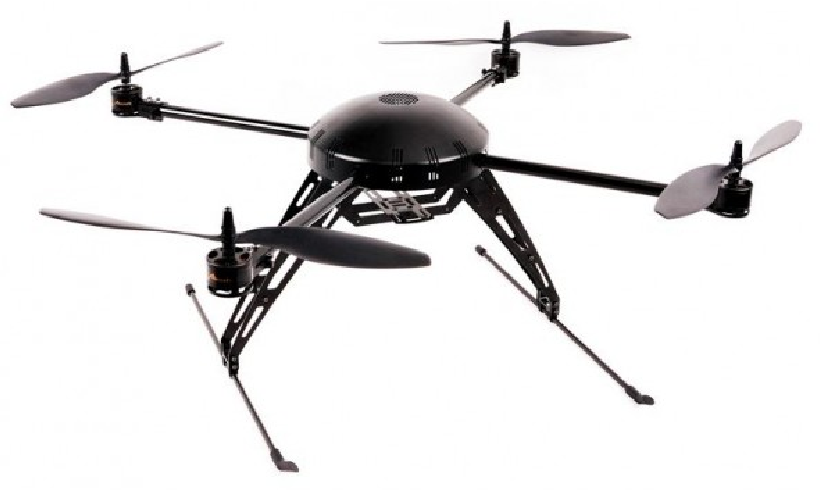
\includegraphics[width=0.36\textwidth]
  			{./pics_eleccion_hardware/aircraft.png}}
  \subfloat[Turbo Ace X720]{\label{fig:turboace} 
  		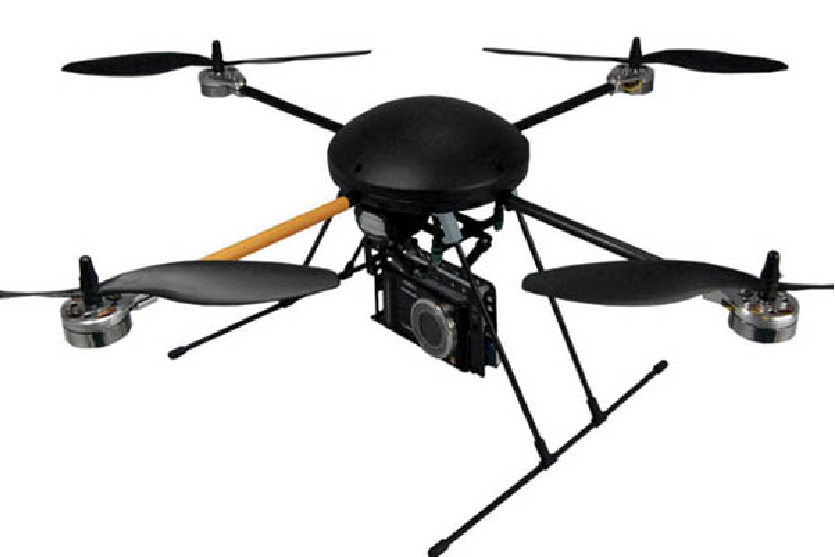
\includegraphics[width=0.32\textwidth]
  			{./pics_eleccion_hardware/turboace.png}}
  \caption{Fotos de las posibles plataformas a utilizar}
  \label{fig:cuadricopteros}
\end{figure}

\subsection{Definici\'on de la plataforma - Cuadric\'opetro}

\begin{itemize}
	\item El \emph{Turbo Ace X720} tiene h\'elices de 12 pulgadas y el grupo h\'elice motor proporciona una eficiencia de $12\,g/W$, superando a los otros dos cuadric\'opteros considerados.
	\item La carga \'util que puede trasportar el \emph{Turbo Ace X720} es la mayor de todos los cuadric\'opteros considerados.
	\item El \emph{Turbo Ace X720} trae un sistema de nivelaci\'on autom\'atica y estabilizaci\'on que resultar\'a \'util al momento de controlarlo con el mando remoto. Adem\'as no incluye excesivas utilidades para este mando, las cuales no ser\'ian utilizadas y contribuir\'ian a encarecer el precio.
\end{itemize}

	Por todas las razones expuestas anteriormente y los an\'alisis comparativos realizados se concluye que la opci\'on que mejor se adec\'ua a nuestro proyecto es el \textbf{Turbo Ace X720}. 

\newpage
\section{Inteligencia}
\vspace*{15pt}

Adem\'as de la plataforma f\'isica, deben seleccionarse componentes electr\'onicos capaces de procesar la informaci\'on proveniente de los sensores, computar y ejecutar los algoritmos de control y generar las se\~nales necesarias para transmitir las instrucciones a los motores.\\
\\
Ser\'a necesario, entonces, seleccionar uno (o varios) componentes capaces de desarrollar las tareas mencionadas. Para ello, el sistema elegido deber\'a contar con:

\begin{itemize}
\item Un microprocesador con suficiente poder de c\'omputo.
\item Un sistema de entradas y salidas que permita interactuar con la instrumentaci\'on y con el sistema de control de motores.
\item Un sistema de memoria no vol\'atil que permita mantener cargado el programa de control.
\item Elementos de comunicaci\'on para establecer conexi\'on con un PC.
\item Un sistema de potencia que brinde energ\'ia al sistema con una autonom\'ia suficiente.
\end{itemize}

Dado que el sistema utilizar\'a motores brushless, es necesario contar con un sistema capaz de generar se\~nales PWM, ya sea mediante software, hardware o ambas, para controlar los motores.\\
\\
Tambi\'en ser\'a necesario que el sistema seleccionado tenga una interfaz UART que permita la comunicaci\'on con los sensores involucrados.\\
\\
Es evidente que la elecci\'on de la inteligencia no puede realizarse en forma independiente, sino que estar\'a fuertemente condicionada por la elecci\'on del resto de la arquitectura del sistema final. Por ello, las decisiones tomadas ser\'an afectadas considerablemente por las caracter\'isticas del resto de los componentes del sistema.\\
\\
%Micro. decir pa q lo usamos, q tiene q hacer. payar
Teniendo en cuenta las restricciones anteriores, se seleccionaron varias arquitecturas posibles en una primera etapa. Se realizo un primer estudio de las diversas posibilidades ofrecidas, manej\'andose varias opciones.\\
\\
Varias de ellas fueron descartadas por no cumplir todos los requisitos arriba mencionados. De la opciones que s\'i verificaban dichos requisitos fueron descartadas aquellas que implicaban m\'as de un componente, opt\'andose por considerar las opciones que fueran capaces de proveer todas las prestaciones arriba mencionadas integradas en una \'unica placa.\\
\\
Una vez realizado un primer an\'alisis de las vastas posibilidades disponibles en el mercado se pre-seleccionaron las siguientes opciones:

\begin{enumerate}
\item Beagleboard XM

\item Gumstix Overo Fire
\end{enumerate}
A continuaci\'on se desarrollar\'an y comparar\'an las caracter\'isticas fundamentales de ambas opciones, permitiendo as\'i la selecci\'on de alguno de ellos en virtud de los requisitos del sistema que se desea implementar. 

\subsection*{Procesadores: CPU y DSP}
Es claro que el procesador es un componente determinante, pues ser\'a el encargado de computar completamente los algoritmos de control. Tambi\'en se encargar\'a de manejar parte de la comunicaci\'on con la instrumentaci\'on y elementos de control. Finalmente, deber\'a ser capaz de manejar informaci\'on proveniente de los canales de comunicaci\'on establecidos con un PC.

\begin{table}[H]
\begin{tabular}{p{130pt}|p{130pt}|p{130pt}|} 
\cline{2-3}
& \cellcolor[gray]{0.8} \textbf{Beagleboard XM} 
& \cellcolor[gray]{0.8} \textbf{Gumstix Overo Fire} \\ \cline{1-3} \hline
\multicolumn{1}{|p{130pt}|}{\cellcolor[gray]{0.8}\textbf{CPU}} 
&ARM Cortex A8 1Ghz,  256KB L2 cache, 1200 MIPS &ARM Cortex A8 720Mhz, 256KB L2 cache, 1200 MIPS \\ 
\hline 
\multicolumn{1}{|p{130pt}|}{\cellcolor[gray]{0.8}\textbf{DSP}} 
&TMS320C64x+, 800Mhz &TMS320C64x+, 520Mhz\\
\hline
\end{tabular}
\caption{Procesadores}
\label{tab:procesadores}
\end{table}

Resulta evidente que ambas opciones presentan los mismos procesadores, con la salvedad que ambos procesadores de la Beagleboard presentan una mayor frecuencia de reloj. 

\subsection*{Memoria}

La memoria disponible en el sistema (tanto est\'atica como vol\'atil) resulta de vital importancia, pues ser\'a all\'i que se guardar\'a la informaci\'on del programa de control, configuraciones, etc. Adicionalmente, es necesario contar con suficiente memoria vol\'atil a la hora de procesar datos y ejecutar los algoritmos de control.\\

\begin{table}[H]
\begin{tabular}{p{130pt}|p{130pt}|p{130pt}|} 
\cline{2-3}
& \cellcolor[gray]{0.8} \textbf{Beagleboard XM} 
& \cellcolor[gray]{0.8} \textbf{Gumstix Overo Fire} \\ \cline{1-3} \hline
\multicolumn{1}{|p{130pt}|}{\cellcolor[gray]{0.8}\textbf{Vol\'atil(RAM)}} 
&512Mb & 256Mb\\ 
\hline 
\multicolumn{1}{|p{130pt}|}{\cellcolor[gray]{0.8}\textbf{Est\'atica}} 
&Sin memoria interna.  Soporta microSD de hasta 4Gb  &256Mb de memoria interna\\
\hline
\end{tabular}
\caption{Memoria}
\label{tab:memoria}
\end{table}

La superioridad de la Beagleboard en cuanto a memoria resulta evidente a partir del an\'alisis anterior.

\subsection*{Dimensiones y peso}

Si bien no resulta una caracetr\'istica determinante, es conveniente que las dimensiones y peso de la placa elegida sean lo menores posibles, de forma de no ocupar gran parte de la carga \'util del cuadric\'optero con electr\'onica asociada a la inteligencia implementada.\\

\begin{table}[H]
\begin{tabular}{p{130pt}|p{130pt}|p{130pt}|} 
\cline{2-3}
& \cellcolor[gray]{0.8} \textbf{Beagleboard XM} 
& \cellcolor[gray]{0.8} \textbf{Gumstix Overo Fire} \\ \cline{1-3} \hline
\multicolumn{1}{|p{130pt}|}{\cellcolor[gray]{0.8}\textbf{Dimensiones}} 
&85.09x87.63mm &17x58mm\\ 
\hline 
\multicolumn{1}{|p{130pt}|}{\cellcolor[gray]{0.8}\textbf{Peso}} 
&36g &5.6g\\
\hline
\end{tabular}
\caption{Dimensiones y Peso}
\label{tab:dim}
\end{table}
En cuanto a dimiensiones y peso, la placa Gumstix Overo Fire parece ser m\'as adecuada.

\subsection*{Programaci\'on y Sistema Operativo}

Es importante tener en cuenta como ser\'a realizada la programaci\'on de los sistemas considerados (d\'onde se almacena el programa, hardware necesario para la programaci\'on, etc.) En particular, es conveniente poder contar con alg\'un sistema operativo que facilite la tareas de programaci\'on, testeo y debugging.

\begin{table}[H]
\begin{tabular}{p{130pt}|p{130pt}|p{130pt}|} 
\cline{2-3}
& \cellcolor[gray]{0.8} \textbf{Beagleboard XM} 
& \cellcolor[gray]{0.8} \textbf{Gumstix Overo Fire} \\ \cline{1-3} \hline
\multicolumn{1}{|p{130pt}|}{\cellcolor[gray]{0.8}\textbf{Sistema Operativo}} 
&Booteable desde microSD &Booteable desde microSD\\ 
\hline 
\multicolumn{1}{|p{130pt}|}{\cellcolor[gray]{0.8}\textbf{Programaci\'on}} 
&A trav\'es de SO. Puerto JTAG de 14 pines &A trav\'es de SO\\
\hline
\end{tabular}
\caption{Programaci\'on y Sistema Operativo}
\label{tab:prog}
\end{table}

Es claro que la placa Beagleboard parece ser mejor en cuanto a sus prestaciones de programaci\'on.

\subsection*{Alimentaci\'on y Energ\'ia}

La forma en que la placa elegida es alimentada, as\'i como el grado de autonom\'ia que pueda lograrse con la misma deben ser tenidos en cuenta.\\
Lograr un nivel de autonom\'ia lo suficientemente grande permitir\'a que el sistema se mantenga en vuelo durante un tiempo mayor. Idealmente, la autonom\'ia de la alimentaci\'on de la inteligencia no deber\'ia ser el factor determinante del tiempo de vuelo del dispositivo.

\begin{table}[H]
\begin{tabular}{p{130pt}|p{130pt}|p{130pt}|} 
\cline{2-3}
& \cellcolor[gray]{0.8} \textbf{Beagleboard XM} 
& \cellcolor[gray]{0.8} \textbf{Gumstix Overo Fire} \\ \cline{1-3} \hline
\multicolumn{1}{|p{130pt}|}{\cellcolor[gray]{0.8}\textbf{Alimentaci\'on}} 
& BeagleJuice. Sistema de alimentaci\'on dise\~nado especificamente para la Beagleboard. (Dimensiones id\'enticas a la misma. Conector est\'andar para BeagleBoard).
& Alimentado desde una Daughter board: Zippy Flightmax 2200mAh 3S1P\\ 
\hline 
\multicolumn{1}{|p{130pt}|}{\cellcolor[gray]{0.8}\textbf{Voltaje. Intensidad de Corriente. Capacidad}} 
&5V, 1.5A, 4500mAh & 11.1V, 44A (= 2200mA x 1P x 20C), 2200mAh 20C\\
\hline
\multicolumn{1}{|p{130pt}|}{\cellcolor[gray]{0.8}\textbf{Autonom\'ia}} 
&6.5 horas &No especificado\\
\hline
\multicolumn{1}{|p{130pt}|}{\cellcolor[gray]{0.8}\textbf{Dimensiones}} 
&85.09x87.63x10mm &102x37x24mm\\
\hline
\multicolumn{1}{|p{130pt}|}{\cellcolor[gray]{0.8}\textbf{Peso}} 
&40g &180g\\
\hline
\end{tabular}
\caption{Alimentaci\'on}
\label{tab:alimentacion}
\end{table}

Pareciera ser evidente que la Beagleboard resulta superior en cuanto a alimentaci\'on disponible, dado que el pack de bater\'ias BeagleJuice fue dise\~nado espec\'ificamente para brindar alimentaci\'on a la misma.

\subsection*{Puertos e I/Os}

Los puertos disponibles para entradas, salidas y/o comunicaci\'on ser\'an tambi\'en un factor determinante a la hora de definir la arquitectura del sistema, pues es imperativo que el sistema de control pueda comunicarse con los sensores, el sistema de control de motores, etc.

\begin{table}[H]
\begin{tabular}{p{130pt}|p{130pt}|p{130pt}|} 
\cline{2-3}
& \cellcolor[gray]{0.8} \textbf{Beagleboard XM} 
& \cellcolor[gray]{0.8} \textbf{Gumstix Overo Fire} \\ \cline{1-3} \hline
\multicolumn{1}{|p{130pt}|}{\cellcolor[gray]{0.8}\textbf{Puertos}} 
&\begin{itemize}
\item 14 pin JTAG
\item UART
\item 28 pin expansion port
\item LCD
\item DVI-D
\item S-VIDEO
\item Stereo in/out
\item USB-OTG
\item RS232
\item EHCI
\item 4 USBs
\item 10/100Mbps Ethernet
\end{itemize}
&\begin{itemize}
\item wifi
\item bluetooth
\item 2x70 pin expansion board port
\item 27 pin camara port
\end{itemize}\\
\hline
\end{tabular}
\caption{Puertos}
\label{tab:puertos}
\end{table}

Cada opci\'on presenta ventajas y desventajas con respecto a los puertos disponibles. Si bien la Beagleboard parece tener una mayor variedad de puertos, la Gumstix Overo Fire cuenta con puertos WiFi y Bluetooth integrados, lo cual resulta ser una ventaja considerable en t\'erminos de comunicaci\'on.

\subsection*{Comunicaci\'on}

Es deseable que el sistema posea alg\'un tipo de comunicaci\'on inal\'ambrica integrada.

\begin{table}[H]
\begin{tabular}{p{130pt}|p{130pt}|p{130pt}|} 
\cline{2-3}
& \cellcolor[gray]{0.8} \textbf{Beagleboard XM} 
& \cellcolor[gray]{0.8} \textbf{Gumstix Overo Fire} \\ \cline{1-3} \hline
\multicolumn{1}{|p{130pt}|}{\cellcolor[gray]{0.8}\textbf{WiFi}} 
&No &S\'i\\ 
\hline 
\multicolumn{1}{|p{130pt}|}{\cellcolor[gray]{0.8}\textbf{Bluetooth}} 
&No &S\'i\\
\hline
\end{tabular}
\caption{Comunicaci\'on}
\label{tab:comunicacion}
\end{table}

La Gumstix Overo Fire resulta claramente superior en este aspecto.

\subsection*{Precio}

El precio resulta ser, evidentemente, un factor importante a tener en cuenta.

\begin{table}[H]
\begin{tabular}{p{130pt}|p{130pt}|p{130pt}|} 
\cline{2-3}
& \cellcolor[gray]{0.8} \textbf{Beagleboard XM} 
& \cellcolor[gray]{0.8} \textbf{Gumstix Overo Fire} \\ \cline{1-3} \hline
\multicolumn{1}{|p{130pt}|}{\cellcolor[gray]{0.8}\textbf{Precio}} 
&149USD &220USD\\
\hline 
\end{tabular}
\caption{Precio}
\label{tab:precio}
\end{table}

Dada la diferencia de precios, ser\'ia deseable utilizar la Beagleboard, siempre y cuando esto no vaya en detrimento del desempe\~no final del sistema.

\subsection*{Otras caracter\'isticas}

Se presentan, a continuaci\'on, algunas caracter\'isticas propias relevantes de cada uno de los sistemas propuestos.

\begin{table}[H]
\begin{tabular}{p{130pt}|p{130pt}|p{130pt}|} 
\cline{2-3}
& \cellcolor[gray]{0.8} \textbf{Beagleboard XM} 
& \cellcolor[gray]{0.8} \textbf{Gumstix Overo Fire} \\ \cline{1-3} \hline
\multicolumn{1}{|p{130pt}|}{\cellcolor[gray]{0.8}\textbf{Otras caracter\'isticas}} 
&\begin{itemize}
\item Existencia de Camera Boards integrables directamente en un puerto dedicado
\item Existencia de la biblioteca OpenCV de visi\'on computacional, optimizada para ser utilizada por Beagleboard
\end{itemize}

&\begin{itemize}
\item Existencia de gran variedad de daughter boards con diversas funcionalidades
\end{itemize}\\ 
\hline 
\end{tabular}
\caption{Otras carater\'isitcas}
\label{tab:otras}
\end{table}

Si se tiene en cuenta el objetivo secundario  planteado (desarrollar un algoritmo de tracking visual), la Beagleboard parece ser m\'as adecuada.

\subsection{Definici\'on de la inteligencia}
\vspace*{15pt}

En virtud del an\'alisis anterior puede asegurarse que:

\begin{itemize}
\item La placa Beagleboard parece ser superior en los siguientes aspectos:
	\subitem Procesadores
	\subitem Memoria
	\subitem Programaci\'on y Sistema Operativo
	\subitem Alimentaci\'on
	\subitem Puertos e I/Os
	\subitem Precio
\item La placa Gumstix Overo Fire parece ser superior en los siguientes aspectos:
	\subitem Dimensiones y Peso
	\subitem Comunicaci\'on
\item Cada placa presenta sus caracter\'isticas \'unicas, lo cual provee ventajas y desventajas para ambas arquitecturas posibles. Si se tiene en cuenta el objetivo secundario del proyecto, it est, la implementaci\'on de un sistema capaz de realizar tracking visual mediante una c\'amara, un sistema basado en la placa Beagleboard parecer\'ia ser m\'as adecuado.
\end{itemize}

Teniendo en cuenta las observaciones anteriores, se opt\'o por construir el sistema en base a una arquitectura basada en la placa Beagleboard.

\newpage
\section{Comunicaci\'on}
\vspace*{15pt}

La inteligencia debe comunicarse con dos bloques del sistema: el de los sensores y el de los motores sobre los cuales se act\'ua. Adem\'as es necesario comunicar a la intelegencia con una PC con el objetivo de programar tanto los algoritmos de control como los rumbos del sistema. 
 
\subsection{Comunicaci\'on con PC}
\vspace*{15pt}
La placa elegida posee diversos puertos USB, por dicho motivo se pueden utilizar dichos puertos para obtener una comunicaci\'on directa con la PC. Dicha comunicaci\'on sirve para programar el sistema en una primera etapa, sin embargo no parece la forma m\'as adecuada de comunicarse con el cuadric\'optero mientras el mismo se encuentra en el aire para reprogamar una ruta, o para modificar alg\'un detalle de un algoritmo. Por dicho motivo se opta por alguna comunicaci\'on de tipo inal\'ambrica. Las opciones que consideradas fueron: WiFi, Bluetooth y GSM. Al poseer en la intelegencia un kernel de linux, la comunicaci\'on v\'ia WiFi es muy sencilla de implementar. Por dicho motivo se opta por este tipo de comunicaci\'on. Al disponer de diversos puertos USB en la inteligencia se opta por un m\'odulo WiFi USB.    


\subsection{Comunicaci\'on con instrumentaci\'on}
\vspace*{15pt}

En lo que respecta a la comunicaci\'on con la instrumentaci\'on se disponen de diversas opciones. Se tiene la posibilidad de comunicarse a trav\'es de un protocolo serie, I2C o incluso puertos USB. Por dicho motivo este aspecto no ser\'a analizado cabalmente en esta secci\'on sino que se realizar\'a al momento de analizar las opciones de comunicaci\'on.  

\subsection{Comunicaci\'on con motores}
\vspace*{15pt}

Los motores, tal como se explic\'o anteriormente, son comandados mediante se\~nales PWM. Por lo tanto, la comunicaci\'on entre la inteligencia y los motores ser\'a cableada. La se\~nal de entrada de los ESCs se conectar\'a directamente a los pines de salida de la inteligencia donde se programen los PWM. 

\newpage
\section{Instrumentaci\'on}
\vspace*{15pt}
Para poder controlar el sistema es importante poder conocer los valores que toman las variables del mismo. Como se ver\'a en el cap\'itulo sobre el desarrollo del modelo f\'isico del cuadric\'optero, las variables que es necesario conocer son:

\begin{itemize}
\item La orientaci\'on del sistema en el sistema de coordenadas utilizado
\item La altura del sistema en el sistema de coordenadas utilizado
\item La aceleraci\'on en las tres coordenadas
\item La velocidad angular del sistema seg\'un tres ejes de rotaci\'on
\end{itemize}

Por dicho motivo parece imprescindible dotar al sistema de sensores capaces de medir dichas magnitudes.

\subsection{Aceler\'ometro}
\label{acelerometro}
\vspace*{15pt}

Previo a definir el aceler\'ometro, su principio b\'asico de funcionamiento y su inter\'es en la aplicaci\'on presentada, se debe realizar una discusi\'on f\'isica sobre la ca\'ida libre como sistema de referencia.\\
En la f\'isica cl\'asica, la fuerza gravitatoria que se ejerce sobre una masa es proporcional a la intensidad del campo gravitatorio en la posici\'on en la cual se encuentra.\\ 
La teor\'ia general de la relatividad es una teor\'ia m\'etrica de la gravitaci\'on. Los fen\'omenos que en la mec\'anica cl\'asica se le atribuyen a la acci\'on de la fuerza de gravedad, corresponden a movimientos inerciales en una geometr\'ia curvada del espacio-tiempo en la teor\'ia de la relatividad general.\\
\\
Por lo tanto, desde el punto de vista de la f\'isica cl\'asica, un sistema de referencia en ca\'ida libre es un sistema acelerado por la fuerza de la gravedad, y como tal, es no inercial.\\
Por el contrario, desde el punto de vista de la f\'isica relativista, el sistema est\'a acelerado en el espacio, pero no en el espacio-tiempo, por lo tanto el sistema de referencia es inercial.\\

Saldada esta discusi\'on se define un aceler\'ometro como un dispositivo capaz de medir su aceleraci\'on propia en el marco de referencia de la ca\'ida libre relativista. Esto implica que el dispositivo no mide siempre su cambio de velocidad en el espacio.\\
Por ejemplo, la medida de un aceler\'ometro en ca\'ida libre ser\'a cero a pesar de que su velocidad crezca, de la misma forma se puede observar que un aceler\'ometro en reposo respecto de la Tierra, no dar\'a una medida nula, sino que por el contrario medir\'a como aceleraci\'on g.\\
\\
% voy a hablar un poco de xq elejimos acelerometros en un chip (costo, peso) as\'i no tengo que explicar el funcionamiento de todos los tipos de aceler\'ometros que son re distintos.
Existen diversos tipos de aceler\'ometro, en este caso se eligi\'o trabajar con un aceler\'ometro contenido en un circuito integrado (tecnolog\'ia MEMS). Las razones de esta elecci\'on son fundamentalmente tama\~no y peso (cr\'iticos en la aplicaci\'on) y econ\'omicos. Los mismos son m\'as peque\~nos, livianos y baratos que otras tecnolog\'ias.\\
Dicho aceler\'ometro procesa las medidas y las convierte a una salida el\'ectrica; la forma de dicha salida depende si el integrado es anal\'ogico o digital.\\
Los aceler\'ometros basados en tecnolog\'ias MEMS miden cambios internos de la transferencia de calor causada por la aceleraci\'on, ofreciendo ventajas significativas sobre el empleo de una estructura tradicional s\'olida de masas de prueba.\\
Ya que la masa de prueba en el dise\~no de los sensores MEMS son mol\'eculas de gas, las estructuras m\'oviles mec\'anicas son eliminadas dentro del aceler\'ometro.\\
\\
%TODO Referencia a MEMS
Un aceler\'ometro de tres ejes no es otra cosa que un aceler\'ometro capaz de medir su aceleraci\'on propia en tres ejes de coordenadas.\\
\\
%TODO capaz que hay que cambiar esto... depende que informaci\'on usemos para realimentar el quad
Resulta fundamental dotar al cuadric\'optero de un aceler\'ometro, el mismo ser\'a utilizado para obtener la aceleraci\'on lineal en cada instante. Integrando esta informaci\'on se puede obtener la velocidad con la que se desplaza el sistema y por ende se puede obtener la posici\'on del mismo conociendo la posici\'on de partida.
Este instrumento no provee toda la informaci\'on necesaria para realizar el control del sistema. El sistema presenta 6 grados de libertad: las tres coordenadas de su centro de masa y los tres \'angulos que determinan su orientaci\'on.
En particular, el aceler\'ometro no detecta giros, por lo tanto es incapaz de aportarnos toda la informaci\'on necesaria. Es imprescindible entonces dotar al cuadric\'optero de un gir\'oscopo. 
 
\subsection{Gir\'oscopo}
\label{giro}
\vspace*{15pt}

Un gir\'oscopo es un instrumento que mide la velocidad angular del sistema en un marco de referencia inercial como el definido en la secci\'on anterior. Las mismas restricciones sobre tama\~no, peso y costos que se aplicaban para el aceler\'ometro se aplican aqu\'i. Por dicho motivo se vuelve a optar por un instrumento de tecnolog\'ia MEMS.\\ 

% Los gir\'oscopos construidos con esta tecnolog\'ia basan su funcionamiento 
%TODO funcionamiento del gir\'oscopo

%TODO exiplicar errores integration drift
Desde el punto de vista te\'orico, procesando la informaci\'on obtenida a partir del aceler\'ometro y del gir\'oscopo se puede conocer en todo momento la posici\'on del sistema y su orientaci\'on a partir de las condiciones iniciales.\\
En la pr\'actica, sin embargo, esto no sucede as\'i. Todas las medidas realizadas tienen un cierto error. Para obtener la orientaci\'on y la posici\'on a cada instante se deben integrar las medidas obtenidas, por lo tanto, se integra tambi\'en el error. Esto produce una acumulaci\'on de errores que afecta de forma considerable el resultado final luego de cierta cantidad de muestras.\\
Parece razonable, entonces, poder cotejar los datos que se obtienen mediante este m\'etodo con datos obtenidos mediante otras fuentes. Es a partir de esta problem\'atica que surge la necesidad de contar con un GPS. Se puede, cada cierto intervalo de tiempo, observar en cuanto difieren los resultados obtenidos integrando las medidas de los sensores con los datos que aporta el GPS, logrando de esta forma corregir los errores debido al \emph{integration drift}.

\subsection{GPS}
\vspace*{15pt}

La elecci\'on del GPS se bas\'o cas\'i totalmente en lograr la simplicidad del sistema. Exist\'ian muchas opciones, placas de diversos tama\~nos, con diversos tama\~nos de antenas, pero todas con similares especificaciones.\\
\\
Las placas candidatas a estar a cargo de la inteligencia contaban con interfaces USB, por lo que se opt\'o por comprar un dongle GPS, cuyas especificaciones son similares a las del resto de las opciones, y se puede comunicar via USB. Existen drivers para dicho GPS en linux, por lo que la comunicaci\'on con el mismo no deber\'ia ser un problema.\\
\\
Se opt\'o por utilizar un GPS \textit{Canmore GT-730F}.

\begin{figure}[h!]
	\centering
	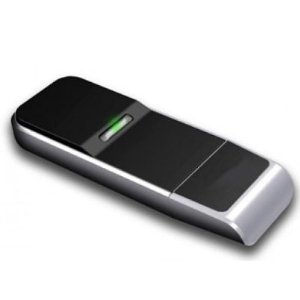
\includegraphics[width=0.2\textwidth]{./pics_eleccion_hardware/gps.jpg}
	\caption{Canmore GT-730F}
	\label{fig:gps}
\end{figure}

\subsection{Sensor de presi\'on}
\vspace*{15pt}
Si bien un dispositivo GPS provee una estimaci\'on de la altura a la que se encuentra, la misma resulta ser poco exacta y confiable, por depender fuertemente de la cantidad de sat\'elites vistos por el GPS as\'i como por el efecto del rebote de las ondas en estructuras cercanas (resulta particularmente cr\'itico el efecto de los rebotes en el piso, los cuales dan poca precisi\'on a la medida de altura al estar muy cerca del suelo). Por este motivo es necesario contar con un sensor de presi\'on absoluta que nos permita determinar la altura del cuadric\'optero en forma independiente al resto de los sensores. La medida de presi\'on debe ser absoluta pues es este tipo de medidas las que pueden ser traducidas a altura en forma r\'apida y confiable.

\subsection{Magnet\'ometro}
\vspace*{15pt}
Si bien el sistema contar\'a con gir\'oscopos que permitir\'an, a trav\'es de integraci\'on, estimar la orientaci\'on del cuadric\'optero, dicha estimaci\'on est\'a sujeta a los errores asociados a este tipo de sensores (errores de drift e integraci\'on, entre otros), siendo adem\'as dicha medida una medida diferencial, teniendo como \'unica referencia la orientaci\'on inicial del cuadric\'optero. Eso por ello que resulta conveniente contar con un magnet\'ometro que permita tener una medida absoulta y confiable de la orientaci\'on del sistema, la cual puede ser entonces complementada y corregida mediante la informaci\'on obtenida mediante la integraci\'on de la informaci\'on generada por el gir\'oscopo.

\subsection{Sensor de temperatura}
\vspace*{15pt}
Si bien el control del sistema no depende directamente de la temperatura, los instrumentos a utilizarse est\'an construidos con cierta tecnolog\'ia que presenta dependencia con (y por ende tendr\'a errores asociados a) la temperatura. El contar con un sensor de temperatura permitir\'a sensar la misma y realizar correcciones en tiempo real que permitan minimizar dicho errores.

\subsection{Definici\'on de instrumentaci\'on}
\vspace*{15pt}


%TODO Aceler\'ometro + gir\'oscopo Pater
En la secciones \ref{acelerometro} y \ref{giro} se detall\'o el porqu\'e de la elecci\'on de la tecnolog\'ia MEMS para el aceler\'ometro y el gir\'oscopo. Las razones fundamentales son el costo, tama\~no y peso de los instrumentos, siendo los \'ultimos dos cr\'iticos en la aplicaci\'on.
A partir de esta definici\'on surgen dos posibilidades, integrar los instrumentos dise\~nando un PCB o adquirir uno en el cual se encuentren los dos sensores. Al dise\~nar un PCB se reduce el costo de la instrumentaci\'on. El precio de cada chip ronda los 5 U\$S, sumado al precio de algunas resistencias, capacitores y otros materiales necesarios para la construcci\'on del PCB (Placa de cobre, percloruro, esta\~no, etc) hacen un total muy inferior al costo de comprar una placa ya armada (m\'as de 60 U\$S). Sin embargo, el proceso de dise\~no del PCB extiende los plazos en gran medida, se debe dise\~nar el circuito, construir y verificar su funcionamiento. El proceso mencionado tendr\'a probablemente una duraci\'on superior a las dos semanas, lo cual implica un retraso en varios aspectos del proyecto, ya que diversas tareas previamente definidas dependen fuertemente del funcionamiento de la instrumentaci\'on. Por otra parte el peso que representa el costo de adquirir una placa en la que se incluyan ambos sensores (aceler\'ometro y gir\'oscopo) en el presupuesto total es muy bajo (4\%).\\
\\
En base al an\'alisis realizado se opta por adquirir una placa ya dise\~nada que contenga los sensores necesarios. Existe una gran diversidad de soluciones de instrumentaci\'on en el mercado. Debido a los requerimientos del proyecto se descartaron muchas de ellas. Las opciones consideradas finalmente se resumen en la siguiente tabla. La caracter\'istica com\'un a todas ellas es que pueden medir 6 grados de libertad, la misma cantidad de variables del sistema a controlar (tres coordenadas correspondientes a la posici\'on del centro de masa, raw, yaw, pitch).\\
\\ %TODO ANEXO.

Los criterios que se fijaron para definir la instrumentaci\'on fueron los siguientes:
\begin{itemize}
\item
Rango de medidas de los sensores
\item
Capacidad de c\'omputo
\item
Facilidad de programaci\'on (algunas placas incluyen microprocesadores)
\item
Comunicaci\'on disponible 
\item
Compatibilidad con el resto del sistema
\item
Costo
\end{itemize}

En lo que respecta al rango de medida de los aceler\'ometros se defini\'o que el mismo fuera de 3g. Dicha elecci\'on est\'a fundamentada en que se planea un vuelo en el cual no se precisen considerar aceleraciones que sean muy superiores a la de la ca\'ida libre.  Asimismo, se defini\'o como rango de medida de los gir\'oscopos un valor  superior a los 300$^o$/s, de forma que el sistema pueda realizar un giro casi completo en cualquiera de los tres ejes en 1 segundo. 
%TODO Masmenos 3g y masomenos 300
Lo que se observa es que todos los aceler\'ometros y giroscopos de las placas de esta preselecci\'on cumplen con dicho requerimiento.


\begin{table}[H]
\begin{tabular}{p{130pt}|p{70pt}|p{65pt}|p{55pt}|p{90pt}|} 
\cline{2-5} 
& \multicolumn{2}{|c|}{\cellcolor[gray]{0.7}\textbf{Aceler\'ometro}} 
& \multicolumn{2}{|c|}{\cellcolor[gray]{0.7}\textbf{Gir\'oscopo}}  \\ \cline{2-5}
& \cellcolor[gray]{0.8} \textbf{Rango} 
& \cellcolor[gray]{0.8} \textbf{Sensibilidad}
& \cellcolor[gray]{0.8} \textbf{Rango} 
& \cellcolor[gray]{0.8} \textbf{Sensibilidad} \\ \cline{2-5} \hline
\multicolumn{1}{|c|}{\cellcolor[gray]{0.8}\textbf{CHR-6d}}
& 3g & 300mV/g &  400$^o$/s \'o 100$^o$/s &  2.5mV/($^o$/s) \'o 2.5mV/($^o$/s) \\ \hline
\multicolumn{1}{|p{130pt}|}{\cellcolor[gray]{0.8}\textbf{Atomic IMU}}
&  1.5g  ;  6g &  800mV/g   200mV/g &  300$^o$/s  &  3.3mV/($^o$/s)\\ \hline
\multicolumn{1}{|p{130pt}|}{\cellcolor[gray]{0.8}\textbf{IMU Digital Combo Board}}
&  2g  ;  16g &  356LSB/g   321LSB/g &  2000$^o$/s  &  14.375 LSB/($^o$/s)\\ \hline
\multicolumn{1}{|p{130pt}|}{\cellcolor[gray]{0.8}\textbf{IMU Analgo Combo Board Razor}}
&  3g &  300mV/g  &  300$^o$/s  1200$^o$/s &  3.3mV/($^o$/s)  0.83mV/($^o$/s)\\ \hline
\multicolumn{1}{|p{130pt}|}{\cellcolor[gray]{0.8}\textbf{IMU Fusion Board}}
&  2g &  256 LSB/g  &  250$^o$/s  2000$^o$/s &  131 LSB/($^o$/s)     16.4 LSB/($^o$/s)\\ \hline
\multicolumn{1}{|p{130pt}|}{\cellcolor[gray]{0.8}\textbf{Mongoose 9DoF IMU}}
&  2g; 4g; 8g; 16g &  256 LSB/g 128 LSB/g 64 LSB/g \emph{} 32 LSB/g  & 2000$^o$/s & 14.375 LSB/($^o$/s)\\
\hline 
\end{tabular}
\caption{Sensores}
\label{tab:sensores}
\end{table}

Resulta conveniente que la instrumentaci\'on posea un microprocesador.\\
La raz\'on principal para esto es que le ahorra tiempo a la inteligencia del sistema en el procesamiento de las medidas crudas de los sensores.\\
Los sensores presentan sus medidas constantemente en forma anal\'ogica o digtal dependiendo del sensor en cuesti\'on. En caso de ser una medida anal\'ogica  la misma debe ser, en primer lugar, digitalizada.\\
Una vez que se tiene la medida digitalizada se debe realizar un procesamiento que consiste b\'asicamente en ponerle una marca de tiempo a cada medida y asociarle una etiqueta correspondiente al sensor que la realiz\'o. \\
%TODO ver si finalmente lo hacemos as\'i
Resulta sumamente interesante que no sea el procesador principal quien se encarga de esta identificaci\'on, sino que el mismo reciba los datos pre-procesados. Por esta raz\'on se favorecieron las placas que incluyeran un microprocesador. 


\begin{table}[H]
\begin{tabular}{p{110pt}|p{65pt}|p{65pt}|p{60pt}|p{60pt}|} 

\cline{2-5} 
& \cellcolor[gray]{0.8} \textbf{Frecuencia reloj} 
& \cellcolor[gray]{0.8} \textbf{Largo de palabra}
& \cellcolor[gray]{0.8} \textbf{RAM} 
& \cellcolor[gray]{0.8} \textbf{Flash}\\ \cline{2-5} \hline
\multicolumn{1}{|p{110pt}|}{\cellcolor[gray]{0.8}\textbf{Mongoose 9DoF IMU}}
&  20MHz &  8 bits &  2Kb &  32Kb \\ \hline
\multicolumn{1}{|p{110pt}|}{\cellcolor[gray]{0.8}\textbf{CHR-6d}}
&  72MHz &  32 bits &  20Kb &  64Kb \\ \hline
\multicolumn{1}{|p{110pt}|}{\cellcolor[gray]{0.8}\textbf{Atomic IMU}}
&  10MHz  &  8 bits &  2Kb  &  32Kb \\ \hline
\multicolumn{1}{|p{110pt}|}{\cellcolor[gray]{0.8}\textbf{IMU Digital Combo Board}}
&  - &  - &  -  &  -\\ \hline
\multicolumn{1}{|p{110pt}|}{\cellcolor[gray]{0.8}\textbf{IMU Analgo Combo Board Razor}}
&  - &  -  &  - &  -\\ \hline
\multicolumn{1}{|p{110pt}|}{\cellcolor[gray]{0.8}\textbf{IMU Fusion Board}}
&  - &  -  &  - &  -\\
\hline 
\end{tabular}
\caption{Caracter\'isticas de los microprocesadores}
\label{tab:micro}
\end{table}

En caso de optar por una placa con microprocesador resulta fundamental que la misma sea sencilla de programar. Las razones son evidentes, ya que si los algoritmos que vienen programados de f\'abrica no resultan adecuados para la aplicaci\'on \'estos deber\'ian poder ser modificados f\'acilmente.\\
Tambi\'en parece importante que el c\'odigo de f\'abrica sea abierto, principalmente para comprender su funcionamiento y poder procesar adecuadamente los datos que se obtengan de los sensores. Es interesante adem\'as poder modificar secciones puntuales de c\'odigo, sin necesidad de reprogramar completamente el microprocesador.\\
\\
La comunicaci\'on no result\'o un factor cr\'itico ya que todos los candidatos a procesador principal poseen diversas interfaces (UART, I2C, Converoares AD). Sin embargo, debido a la familiarizaci\'on del grupo de proyecto con las comunicaciones serie, se prefiri\'o dar prioridad a aquellas placas que se comunicaran via UART (en caso de que se optara por una placa con microprocesador).\\
\\
En lo que respecta a compatibilidad con el sistema, se busc\'o que la alimentaci\'on de la placa fuera la misma que la del procesador principal. Por dicha raz\'on lo ideal ser\'ia que la placa pueda ser alimentada a 5V.\\
\\
A partir de las consideraciones anteriores, se consider\'o inicialmente que la soluci\'on m\'as adecuada para el objetivo que se plantea en esta secci\'on es la placa \emph{Razor Atomic IMU}.\\
Dicha placa cumple con los rangos de medida especificados anteriormente y posee un procesador de 8 bits con un reloj de 10MHz.\\
Existen ya scripts en C disponibles para programar el dispositivo. Los mismos pueden ser modificados en caso de no cumplir con todos los requerimientos necesarios.\\
La placa dispone de un puerto JTAG para programaci\'on.\\
La forma que tiene la placa de presentar los datos obtenidos de los sensores es a trav\'es de un puerto serie capaz de transmitir datos con una tasa de transferencia de 115.200bps.\\
Cabe aclarar que la Atomic IMU es la \'unica de las soluciones consideradas que puede ser alimentada con una fuente de tensi\'on de 5V.\\
Finalmente, el costo de la misma es de los m\'as bajos dentro de las posibilidades consideradas.

En la figura \ref{fig:IMU} se puede observar dicha placa de instrumentaci\'on:

\begin{figure}[H]
	\centering
	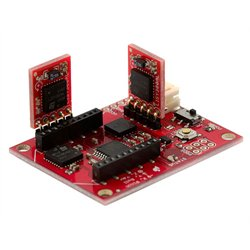
\includegraphics[width=0.3\textwidth]{./pics_eleccion_hardware/IMU.jpg}
	\caption{Atomic IMU}
	\label{fig:IMU}
\end{figure}

Luego de seleccionada y adquirida la placa, y a partir de varias pruebas realizadas y conocimientos adquiridos a lo largo del desarrollo del proyecto resulto claro que la misma no pose\'ia suficiente cantidad de sensores para la aplicaci\'on deseada.\\
\\
A partir de este punto se procedi\'o a estudiar los nuevos requierimientos en cuanto a sensores y resulto evidente que adem\'as de los sensores ya existentes en la placa seleccionada ser\'ia necesario a\~nadir un magnet\'ometro y un sensor de presi\'on.\\
\\
Nuevamente se plante\'o la disyuntiva entre comprar otra placa que contenga todos los sensores ya integrados o a\~nadir los nuevos sensores en forma independiente. Con argumentos similares a los que motivaron la primer compra se opt\'o por adquirir una nueva placa.\\
\\
Analizando las diversas opciones se opt\'o por adquirir la Mongoose 9DoF IMU. La misma no s\'olo cuenta con un magnet\'ometro y un sensor de presi\'on adecuados a los requerimientos de la aplicaci\'on, sino que resulta ser considerablemente similar a la Atomic IMU, presentando mejores rangos y sensibilidades en sus sensores y mayor capacidad de almacenamiento y procesamiento de datos.\\
Adicionalmente, la Mongoose 9DoF IMU posee un sensor de temperatura que permitir\'a llevar a cabo compensaci\'on por temperatura y corregir las medidas obtenidas a partir de los otros sensores.\\
\\
En la figura \ref{fig:Mongoose} se puede observar dicha placa de instrumentaci\'on:

\begin{figure}[H]
	\centering
	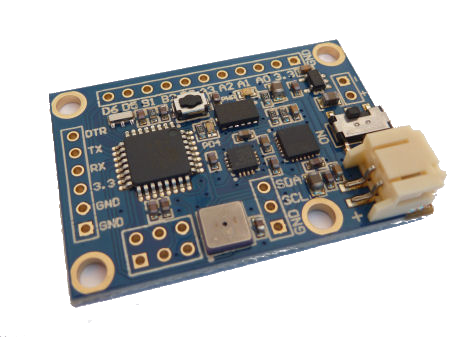
\includegraphics[width=0.3\textwidth]{./pics_eleccion_hardware/Mongoose.png}
	\caption{Atomic IMU}
	\label{fig:Mongoose}
\end{figure}

\newpage
\subsection{Especificaciones t\'ecnicas de la placa de instrumentaci\'on seleccionada (Mongoose 9DoF IMU)}
\vspace*{15pt}

\subsubsection{Aceler\'ometro}

\begin{table}[H]
\begin{center}
\rowcolors{1}{gray!20}{}
\begin{tabular}{|p{3cm}|p{6.5cm}|}
\hline
Rango & $\pm$16g \\
\hline
Resoluci\'on & 10-13 bits (siempre 4mg/LSB) \\
\hline
Datos nuevos &  0.1 a 800 Hz\\
\hline
Ru\'ido XY & 0.75@100Hz - 3@3200Hz LSB-rms\\
\hline
Ru\'ido Z & 1.1@100Hz - 4.5@3200Hz LSB-rms\\
\hline
Cross Axis & $\pm$ 1\% \\
\hline
\end{tabular}
\label{tab:acc}
\end{center}
\end{table}

\textbf{NOTAS}:
\begin{itemize}
\item Output data rate puede llegar a 3200Hz, pero usando SPI. Con I$^2$C a 400kHz solamente se puede llegar a 800Hz.
\item Ancho de banda = $Datos\_nuevos/2$
\end{itemize}

\subsubsection{Gir\'oscopo}

\begin{table}[H]
\begin{center}
\rowcolors{1}{gray!20}{}
\begin{tabular}{|p{3cm}|p{6.5cm}|}
\hline
Rango & $\pm$2000$^\circ/s$ \\
\hline
Resoluci\'on & 14.475 LSB/($^\circ/s$) \\
\hline
Datos nuevos &  3.9Hz a 8kHz\\
\hline
Ancho de banda & 256Hz \\
\hline
Cross Axis & $\pm$ 2\% \\
\hline
Ru\'ido & 0.38 $^\circ/s$-rms \\
\hline
\end{tabular}
\label{tab:gyro}
\end{center}
\end{table}

\textbf{NOTAS}:
\begin{itemize}
\item Datos nuevos: La muestras pasan por un LPF digital de 256 a 5Hz, esto limita el ancho de banda.
\end{itemize}

\subsubsection{Magnet\'ometro}

\begin{table}[H]
\begin{center}
\rowcolors{1}{gray!20}{}
\begin{tabular}{|p{3cm}|p{6.5cm}|}
\hline
Rango & $\pm$8 Ga\\
\hline
Resoluci\'on &  5mGa@GN=2\\
\hline
Datos nuevos &  0.75 - 75Hz\\
\hline
Ancho de banda &  37Hz\\
\hline
Cross Axis & $\pm$0.2\% FS/Ga \\
\hline
Ru\'ido & - \\
\hline
\end{tabular}
\label{tab:magn}
\end{center}
\end{table}

\newpage
\textbf{NOTAS}:
\begin{itemize}
\item El rango queda determinado por la ganancia, que se configura con 3 bits:
\begin{table}[H]
\begin{center}
\rowcolors{1}{gray!20}{}
\begin{tabular}{|c|c|c|c|c|c|c|c|c|}
\hline
\textbf{GN} & 0 & 1 & 2 & 3 & 4 & 5 & 6 & 7 \\
\textbf{Rango} (Ga)& $\pm$0.88 & $\pm$1.3 & $\pm$1.9 & $\pm$2.5 & $\pm$4.0 & $\pm$4.7 & $\pm$5.6 & $\pm$8.1 \\
\hline
\end{tabular}
\label{tab:magn-gain}
\end{center}
\end{table}
\item Se puede configurar para que el dato que muestre sea el promedio de hasta 8 muestras.
\end{itemize}

\subsubsection{Sensor de presi\'on}

\begin{table}[H]
\begin{center}
\rowcolors{1}{gray!20}{}
\begin{tabular}{|p{3cm}|p{6.5cm}|}
\hline
Rango & 300 a 1100 hPa (9000 a -500m)\\
\hline
Resoluci\'on &  1Pa\\
\hline
Precisi\'on. Abs. & typ/max $\pm$1.0/$\pm$3.0 hPa \\
\hline
Precisi\'on Rel. & $\pm$0.5 hPa \\
\hline
Datos nuevos &  typ/max: 3/4.5ms - 17/25ms\\
\hline
Ancho de banda &  333/40Hz\\
\hline
Ru\'ido (hPa) &  0.06 - 0.03\\
\hline
Ru\'ido (m) & 0.5 - 0.25 \\
\hline
\end{tabular}
\label{tab:barometro}
\end{center}
\end{table}

\textbf{NOTAS}:
\begin{itemize}
\item El rango, en altura, se refiere a la altura sobre el nivel del mar.
\item El modo de operaci\'on (cantidad de muestras promediadas) afecta:
  \begin{itemize}
  \item El tiempo de conversi\'on.
  \item El ancho de banda.
  \item La resoluci\'on.
  \item El ru\'ido.
  \end{itemize}
\item Es necesario hacer una medida de temperatura de vez en cuando (1Hz) para mejorar la lectura del sensor de presi\'on.
\end{itemize}

\subsubsection{Sensor de temperatura}

\begin{table}[H]
\begin{center}
\rowcolors{1}{gray!20}{}
\begin{tabular}{|p{3cm}|p{6.5cm}|}
\hline
Rango & 0 a 65 $^\circ$C\\
\hline
Resoluci\'on &  0.1 $^\circ$C\\
\hline
Precisi\'on Abs. & typ/max $\pm$1.0/$\pm$2.0 $^\circ$C\\
\hline
Datos nuevos &  typ/max: 3/4.5ms\\
\hline
Ru\'ido & - \\
\hline
\end{tabular}
\label{tab:temp}
\end{center}
\end{table}

\textbf{NOTAS}:
\begin{itemize}
\item El sensor de temperatura est\'a incorporado al sensor de presi\'on.
\end{itemize}


\end{document}

%Algunos layouts para poner im\'agnenes. Copien y peguen nom\'as. Hay figura com\'un, dos figuras en 1 onda fig 3a y 3b, wrapfigures y una matriz de figuras. Ta bueno, todas quedan lindas y andan bien.
%
%\begin{figure}[h!]
%	\centering
%	\includegraphics[width=0.75\textwidth]{./pics_eleccion_hardware/		.eps}
%	\caption{		}
%	\label{fig:		}
%\end{figure}
%
%\begin{figure} [h!]
%  \centering
%  \subfloat[caption 1]{\label{fig:		}
%  		\includegraphics[width=0.45\textwidth]
%  			{./pics_eleccion_hardware/		.eps}}
%  \subfloat[caption 2]{\label{fig:		} 
%  		\includegraphics[width=0.45\textwidth]
%  			{./pics_eleccion_hardware/ 		.eps}}
%  \caption{Caption general}
%  \label{fig:	label general	}
%\end{figure}
%
%\begin{wrapfigure}{l}{0.6\textwidth}
%  \vspace{-20pt}
%  \begin{center}
%    \includegraphics[width=0.45\textwidth]
%    	{./pics_eleccion_hardware/		.eps}
%  \end{center}
%  \vspace{-20pt}
%  \caption{		}
%  \label{ 		}
%  \vspace{-10pt}
%\end{wrapfigure}
%
%\begin{figure} [h!]
%  \begin{center}
%    \begin{tabular}{cc}
%      \resizebox{50mm}{!}
%      	{\includegraphics{./pics_eleccion_hardware/ 	.eps}} &
%      \resizebox{50mm}{!}
%      	{\includegraphics{./pics_eleccion_hardware/	.eps}} \\
%      \resizebox{50mm}{!}
%      	{\includegraphics{./pics_eleccion_hardware/	.eps}} &
%      \resizebox{50mm}{!}
%      	{\includegraphics{./pics_eleccion_hardware/	.eps}} \\
%    \end{tabular}
%    \caption{ 		}
%    \label{ 		}
%  \end{center}
%\end{figure}